\documentclass[12pt]{article}
\usepackage{amsmath}
\usepackage{tikz}
\begin{document}
\title{Computer Science 181, Homework 2}
\date{April 16th, 2018}
\author{Michael Wu\\UID: 404751542}
\maketitle

\section*{Postponed Problem 2}

\paragraph{d)}

\[\{0,00,01,000,011,1,10,11,100,111\}\]
I have chosen to include the empty string \(\epsilon\) in \(L_b\), which is why \(0\) and \(1\) are in this concatenation.

\paragraph{e)}

\[\{\}\]

\section*{Postponed Problem 6}

This is the set \(S\) of all strings \(s\) over \(\Sigma=\{0,1\}\) which have at least two \(1\)'s and ends in \(1\).

\section*{Problem 0}

\paragraph{a)}

I would interpret this as recursing from the end of the string. The notation implies that the function gets the previous state
from recursively applying the transition function \(\delta^*\) to the prefix string consisting of everything except the last character in the string.
Then it applies \(\delta\) to the last character and the previous state to get the final state. In our old definition, we imply that the function recurses
from the beginning of the string. First it applies the transition function \(\delta\) to the first element of the string and the starting state to get the
next state. Then it calls \(\delta^*\) on the remainder of the string and the next state, which begins the recursion. This recursion ends when no more characters
are remaining in the string, and returns the final state.

\paragraph{b)}

Consider an arbitrary string of length \(n\)
\[x=x_0x_1\ldots x_n\]
such that
\[\forall i\in \{0,1,\ldots,n\} \enspace x_i\in\Sigma\]
Then using our new definition of \(\delta^*(q,x)\) we have
\[\delta^*(q,x)=\delta(\delta^*(q,x_0x_1\ldots x_{n-1}), x_n)\]
which has a base case of \(\delta^*(q,x_0)=\delta(q,x_0)\). Thus through induction we have
\[\delta^*(q,x)=\delta(\delta(\ldots\delta(\delta(q,x_0),x_1)\ldots,x_{n-1}), x_n)\]
Using our old definition of \(\delta^*(q,x)\) we have
\[\delta^*(q,x)=\delta^*(\delta(q,x_0),x_1\ldots x_n)\]
which we expand by continually adding an inner \(\delta\) and moving the first character from the second
element of \(\delta^*\) inside a parenthesis. Thus induction also gives us
\[\delta^*(q,x)=\delta(\delta(\ldots\delta(\delta(q,x_0),x_1)\ldots,x_{n-1}), x_n)\]
This is the exact same result given by the new definition of \(\delta^*\), so the definitions are equivalent.

\section*{Problem 1}

\paragraph{a)}

\[
        \begin{array}{c|c|c}
                (x,y) & q & \delta((x,y),q)\\
                \hline
                (0,0) & a & (1,0)\\
                (0,0) & b & (0,1)\\
                (0,1) & a & (1,1)\\
                (0,1) & b & (0,0)\\
                (1,0) & a & (0,0)\\
                (1,0) & b & (1,1)\\
                (1,1) & a & (0,1)\\
                (1,1) & b & (1,0)
        \end{array}
\]

\paragraph{b)}

\begin{center}
        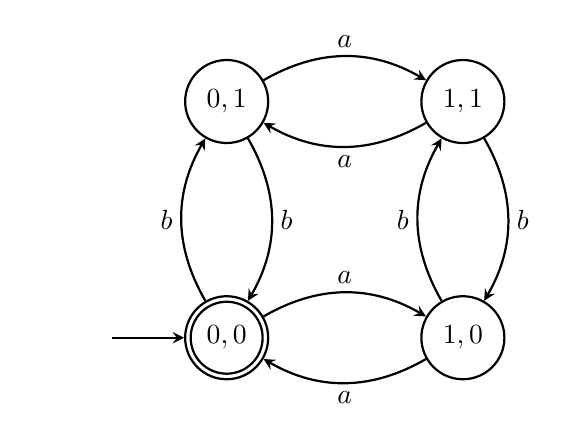
\begin{tikzpicture}
                \begin{scope}[auto, every node/.style={thick, draw,circle,minimum size=3em,inner sep=1}]
                        \node [draw=none] (I) at (-2,0) {};
                        \node (00) at (0,0) {\(0,0\)};
                        \draw[black, thick] (0,0) circle [radius=1.3em];
                        \node (01) at (0,3) {\(0,1\)};
                        \node (10) at (3,0) {\(1,0\)};
                        \node (11) at (3,3) {\(1,1\)};
                \end{scope}

                \begin{scope}[auto, every node/.style={minimum size=1em,inner sep=1}, every path/.style={thick, ->, >=stealth}]
                        \path (I) edge (00);
                        \path (00) edge [bend left] node {\(a\)} (10);
                        \path (01) edge [bend left] node {\(a\)} (11);
                        \path (10) edge [bend left] node {\(a\)} (00);
                        \path (11) edge [bend left] node {\(a\)} (01);
                        \path (00) edge [bend left] node {\(b\)} (01);
                        \path (01) edge [bend left] node {\(b\)} (00);
                        \path (10) edge [bend left] node {\(b\)} (11);
                        \path (11) edge [bend left] node {\(b\)} (10);
               \end{scope}
        \end{tikzpicture}
\end{center}

\paragraph{c)}

This is the set \(S\) of all strings \(s\) over \(\Sigma=\{a,b\}\) which has an even number of \(a\)'s and an even number of \(b\)'s.

\paragraph{d)}

I would interpret the pair \((x,y)\) using the following rules.
\begin{align*}
        \text{even number of } a \text{'s if } & x=0\\
        \text{odd number of } a \text{'s if } & x=1\\
        \text{even number of } b \text{'s if } & y=0\\
        \text{odd number of } b \text{'s if } & y=1
\end{align*}
This allows us to interpret the corresponding names of the states in \(Q\).

\section*{Problem 2}

\begin{center}
        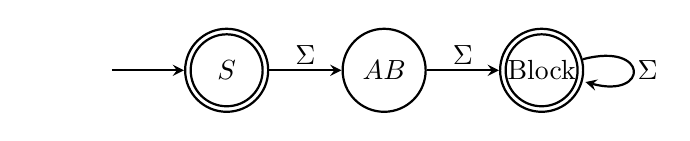
\begin{tikzpicture}
                \begin{scope}[auto, every node/.style={thick, draw,circle,minimum size=3em,inner sep=1}]
                        \node [draw=none] (I) at (-2,0) {};
                        \node (S) at (0,0) {\(S\)};
                        \draw[black, thick] (0,0) circle [radius=1.3em];
                        \node (AB) at (2,0) {\(AB\)};
                        \node (Bl) at (4,0) {Block};
                        \draw[black, thick] (4,0) circle [radius=1.3em];
                \end{scope}

                \begin{scope}[auto, every node/.style={minimum size=1em,inner sep=1}, every path/.style={thick, ->, >=stealth}]
                        \path (I) edge (S);
                        \path (S) edge node {\(\Sigma\)} (AB);
                        \path (AB) edge node {\(\Sigma\)} (Bl);
                        \path (Bl) edge [loop right] node {\(\Sigma\)} (Bl);
               \end{scope}
        \end{tikzpicture}
\end{center}

\section*{Problem 3}

\begin{center}
        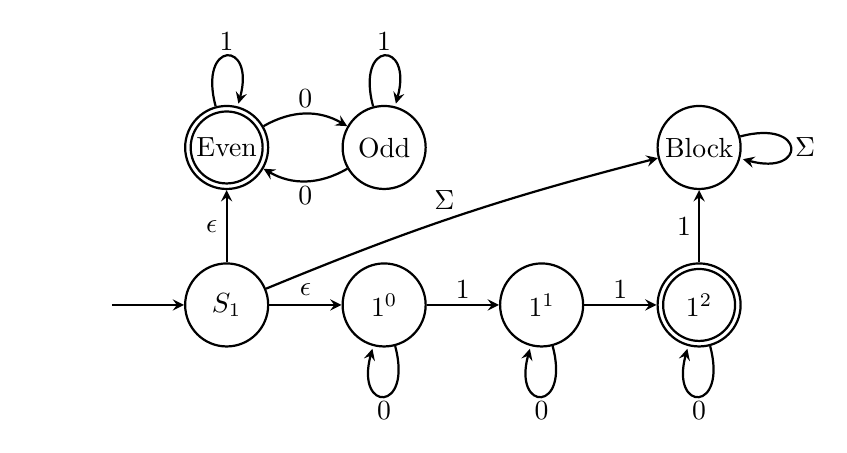
\begin{tikzpicture}
                \begin{scope}[auto, every node/.style={thick, draw,circle,minimum size=3em,inner sep=1}]
                        \node [draw=none] (I) at (-2,0) {};
                        \node (S) at (0,0) {\(S_1\)};
                        \node (E) at (0,2) {Even};
                        \draw[black, thick] (0,2) circle [radius=1.3em];
                        \node (Od) at (2,2) {Odd};
                        \node (0) at (2,0) {\(1^0\)};
                        \node (1) at (4,0) {\(1^1\)};
                        \node (2) at (6,0) {\(1^2\)};
                        \draw[black, thick] (6,0) circle [radius=1.3em];
                        \node (Bl) at (6,2) {Block};
                \end{scope}

                \begin{scope}[auto, every node/.style={minimum size=1em,inner sep=1}, every path/.style={thick, ->, >=stealth}]
                        \path (I) edge (S);
                        \path (S) edge node {\(\epsilon\)} (E);
                        \path (S) edge node {\(\epsilon\)} (0);
                        \path (S) edge [bend left=4] node {\(\Sigma\)} (Bl);
                        \path (E) edge [loop above] node {\(1\)} (E);
                        \path (Od) edge [loop above] node {\(1\)} (Od);
                        \path (E) edge [bend left] node {\(0\)} (Od);
                        \path (Od) edge [bend left] node {\(0\)} (E);
                        \path (0) edge [loop below] node {\(0\)} (0);
                        \path (1) edge [loop below] node {\(0\)} (1);
                        \path (2) edge [loop below] node {\(0\)} (2);
                        \path (0) edge node {\(1\)} (1);
                        \path (1) edge node {\(1\)} (2);
                        \path (2) edge node {\(1\)} (Bl);
                        \path (Bl) edge [loop right] node {\(\Sigma\)} (Bl);
               \end{scope}
        \end{tikzpicture}
\end{center}
If the NFA can be not fully specified, this can be achieved with \(6\) states. Otherwise only using \(6\) states is not possible because
both conditions require checking from the beginning of the string, and so no characters must be consumed before choosing a
condition to validate. So there must be one starting state with two empty transitions, as shown above. The check for an even number
of \(0\)'s requires two states, and the check for exactly two \(1\)'s requires three states. With the addition of a block state, there
must be at least \(7\) states.

\section*{Problem 4}

Two strings in the language are \(bb\) and \(bab\). Two strings not in the language are \(\epsilon\) and \(b\).

\section*{Problem 5}

The set of finite state languages is closed under homomorphisms on the language's alphabet \(\Sigma\). Therefore, \(L_\text{five}\) is a
finite state language if and only if every homomorphism on \(\Sigma=\{a, b, c\}\) results in a finite state language when applied
to \(L_\text{five}\). But the homomorphism
\[h(a)=a \qquad h(b)=b \qquad h(c)=\epsilon\]
yields \(h(L_\text{five})=L_\text{NFS}\), which is not a finite state language. Therefore \(L_\text{five}\) cannot be a finite
state language.

\end{document}